\apendice{Manual del programador} % usar el término que mejor se corresponda.

\section{Estructura de directorios}

Todos los directorios mencionados a continuación, se encuentran en el repositorio de GitHub \textbf {TFG-Numonia-RedesNeuronales} \footnote{\url{https://github.com/NuriaMartinez/TFG-Numonia-RedesNeuronales}}, el cual, está compartido con el tribunal de este TFG.
\begin{itemize}
    
    \item \textbf{README.md}: documento escrito en formato \textit {Markdown}, el cual incluye el resumen del trabajo, una pequeña explicación general del contenido del respositorio de GitHub y una breve descripción acerca de los datos empleados para este trabajo, además de los links a \textit{onedrive}  para descargarse las carpetas ``data'' y ``data\_nuevo''. Ya que, al tratarse de una gran cantidad de imágenes es necesario compartirlo de esta forma. Las carpetas se encuentras comprimidas en \textit{zip}, por lo que, una vez descargadas, antes de empezar a trabajar con ellas, es necesario descomprimirlas.
    \begin{itemize}
        \item \textbf{Carpeta ``data''}: carpeta descargada de internet que incluye tres subcarpetas (``\textit{train}'', ``\textit{test}'' y ``val'') y, estas a su vez incluyen dos subcarpetas (``NORMAL'' y ``PNEUMONIA'') con todas las imágenes de CXT con las que se trabaja en este proyecto.
        \item \textbf{Carpeta ``data\_nuevo''}: tal y como se explica en el \textit{Anexo D}, la carpeta ``data'' no contiene una distribución correcta para trabajar con las imágenes por lo que, empleando Python, se ha creado una nueva carpeta denominada ``data\_nuevo'' con las imágenes distribuidas de una forma proporcional para trabajar correctamente con ellas.
    \end{itemize}
    
    \item \textbf{Carpeta ``codigo''}: en esta carpeta se incluyen los dos \textit{notebooks} de Python y el archivo.py donde se ha realizado toda la parte de programación. Para más información consultar el \textit{Anexo B}. Además, también se encuentra la carpeta ``pics'', con las imágenes incluidas a modo decorativo en los distintos \textit{notebooks} y README.md de GitHub y una serie de carpetas obtenidas a partir de la ejecución de los \textit{notebooks}. 
    
    Debido al espacio limitado de GitHub, no es posible incluir directamente en el repositorio las carpetas generadas automáticamente al ejecutar el código. Por lo tanto, se ha creado un archivo README.md con los enlaces a dichas carpetas comprimidas a través de \textit{OneDrive}. Para acceder a su contenido, bastará con descargarlas y descomprimirlas. Las carpetas incluidas en estos enlaces son:
    
    \begin{itemize}
        \item \textbf{Carpeta ``Datos''}: en esta carpeta se incluyen 5 archivos en formato csv, los cuales se corresponden con los distintos \textit{dataframes} obtenidos en la primera función \textit{``redestribucion\_imagenes''}. En la cual, se busca redistribuir las imágenes de la carpeta \textit{data} de una forma más equitativa. Todos los csv están formados por dos columnas ``nombres\_ficheros'' que corresponde con el nombre de las imágenes y ``clases'' que puede ser un 1 o un 0 en función si la imagen tiene neumonía o no. 
        \begin{itemize}
            \item En el csv denominado \textit{\textbf{dataset\_info}} se muestra el nombre de todas las imágenes existentes en la carpeta data con su correspondiente clase (0 o 1). 
            \item El csv \textit{\textbf{test\_dataset\_info}} se corresponde con la proporción de imágenes seleccionadas para \textit{test}, es decir el 20\% del csv \textit{dataset\_info}, existiendo una proporción entre las clases. 
            \item El csv \textit{\textbf{train\_dataset\_info}} se corresponde con el 80\% del csv \textit{dataset\_info} ya que, antes de obtener la proporción de \textit{train} final, se realiza una distribución de 80/20 para \textit{train} y para \textit{test} y, posteriormente, el 80\% de \textit{train} se divide entre \textit{train} y \textit{val} para obtener la proporción final. Por lo que, se podría decir que, este csv forma parte del proceso de la realización de la función \textit{``redestribucion\_imagenes''} pero no se emplea para la redistribución definitiva.
            \item El csv \textit{\textbf{train\_final\_dataset\_info}} es el \textit{dataframe} final de \textit{train}. Se corresponde con una proporción del 64\% del csv \textit{dataset\_info} con una proporción entre las clases.
            \item Por último, el csv \textit{\textbf{val\_dataset\_info}} se corresponde con una proporción del 16\% del csv \textit{dataset\_info}. También existe una proporción entre las clases.
        \end{itemize}
        \item \textbf{Carpeta ``Historicos''}: en esta carpeta se incluyen diversas subcarpetas, cada una de ellas perteneciente a un modelo o \textit{batch size} determinado para CNN propia o CNN Alex Net y para distinto número de neuronas. Dentro de cada subcarpeta, se encuentran distintos csv obtenidos para cada uno de esos casos. En estos csv se incluyen los valores de diferentes métricas obtenidas durante el entrenamiento en cada época para ese modelo, \textit{batch size} o número de neuronas concretos.
        \begin{itemize}
            \item Los csv dentro de la carpeta denominada\\ \textit{\textbf{historico\_propia\_arqu\_batchsize}} se corresponden con las métricas obtenidas para cada época durante el entrenamiento de los modelos Simple1, Simple2 y Simple3 y los valores de \textit{batch size} 8, 16, 20, 32 y 64 con la CNN propia.
            \item Los csv dentro de la carpeta denominada\\ \textit{\textbf{historico\_alexnet\_arqu\_batchsize}} se corresponden con las métricas obtenidas para cada época durante el entrenamiento de los modelos Simple1, Simple2 y Simple3 y los valores de \textit{batch size} 8, 16, 20, 32 y 64 con la CNN de AlexNet.
            \item Los csv dentro de la carpeta denominada\\ \textit{\textbf{historico\_neuronas}} se corresponden con las métricas obtenidas para cada época durante el entrenamiento del modelo Simple3, basado en la CNN de AlexNet y un \textit{batch size} de 64 con distintos números de neuronas en la capa oculta (512, 1024 y 2048). 
            
        \end{itemize}
        Estos csv han sido obtenidos a partir de la ejecución realizada en el \textit{notebook} ``redes neuronales - neumonia''.
        \item \textbf{Carpeta ``Historicos\_Py''}: La explicación para todos los archivos que se encuentran en esta carpeta coincide con la explicación de la carpeta anterior excepto por un detalle. Y es que, todos los archivos de la carpeta ``Historicos\_Py'' se corresponden con la ejecución realizada en el \textit{notebook} ``redes neuronales ejecución archivo.py''. 
        
        La distinción entre estas dos carpetas se debe a que, los resultados de la ejecución en ambos \textit{notebooks} pueden ser sutilmente diferentes debido a la aleatoriedad de pesos y muestras iniciales en cada ejecución (explicado en el apartado de ``\textit{Resultados} de la memoria). Por lo que, los csv almacenados en dichas carpetas también son distintos.
        
        \item \textbf{Carpeta ``Modelos''}: en esta carpeta, al igual que ocurría con la carpeta ``Historicos'', se incluyen diversas subcarpetas, cada una de ellas perteneciente a un modelo o \textit{batch size} determinado para CNN propia o CNN Alex Net y para distinto número de neuronas. Dentro de cada subcarpeta, se encuentran distintos archivos obtenidos para cada modelo y cada \textit{batch size} de la CNN propia, de la CNN Alexnet y para distinto número de neuronas del modelo Simple3 y \textit{bacht size} 64. 

        \begin{itemize}
            \item Los archivos dentro de la carpeta denominada\\ \textit{\textbf{modelo\_propia\_arqu\_batchsize}} se corresponden con los modelos obtenidos durante el entrenamiento de la arquitectura Simple1, Simple2 y Simple3 y los valores de \textit{batch size} 8, 16, 20, 32 y 64 con la CNN propia.
            \item Los archivos dentro de la carpeta denominada\\ \textit{\textbf{modelo\_alexnet\_arqu\_batchsize}} se corresponden con los modelos obtenidos durante el entrenamiento de la arquitectura Simple1, Simple2 y Simple3 y los valores de \textit{batch size} 8, 16, 20, 32 y 64 con la CNN de AlexNet.
            \item Los archivos dentro de la carpeta denominada\\ \textit{\textbf{modelo\_neuronas}} se corresponden con los modelos obtenidos durante el entrenamiento de la arquitectura Simple3, basado en la CNN de AlexNet y un batch size de 64 con distintos números de neuronas en la capa oculta (512, 1024 y 2048). 
            
        \end{itemize}
    
        Estos archivos, se encuentran en un formato HDF, el cual se emplea para almacenar grandes cantidades de datos (numéricos, gráficos y de texto) de una forma jerárquica, por lo que, la gestión de estos datos se realiza de una forma eficiente \cite{filext24}. 
    
        Dentro de cada archivo, se encuentran los valores de pesos del modelo, su estructura completa (capas, conexiones, etc.), información sobre el optimizador y su estado y la configuración de compilación del modelo que incluye la función de pérdida y las métricas \cite{TensorFlowSave24}.
    
        Al igual que ocurría en el caso anterior, en esta carpeta se guardan los archivos referidos al \textit{notebook} ``redes neuronales - neumonia''.
        \item \textbf{Carpeta ``Modelos\_Py''}: con esta carpeta ocurre exactamente lo mismo que con la carpeta ``Historicos\_Py''. Toda la explicación de cada uno de sus archivos coincide con la ya detallada en la carpeta ``Modelos'' pero, con la diferencia de que, los archivos de esta carpeta se obtienen a partir de la ejecución \textit{notebook} ``redes neuronales ejecución archivo.py''. 
    
        \item \textbf{Carpeta ``Resultados''}: en esta carpeta se incluyen los distintos \textit{dataframes} en formato csv donde se muestran las tablas comparativas obtenidas en este trabajo. 
        \begin{itemize}
            \item El archivo \textit{\textbf{compara\_propia\_arqu\_batch\_def.csv}} se corresponde con la tabla final obtenida tras el entrenamiento de la arquitectura Simple1, Simple2 y Simple3 y los valores de \textit{batch size} 8, 16, 20, 32 y 64 con la CNN propia. Se observan los valores de distintas métricas para cada arquitectura y cada valor de \textit{batch size}.
            \item El archivo \textit{\textbf{compara\_alexNet\_arqu\_batch\_def.csv}} se corresponde con la tabla final obtenida tras el entrenamiento de la arquitectura Simple1, Simple2 y Simple3 y los valores de \textit{batch size} 8, 16, 20, 32 y 64 con la CNN AlexNet. Se observan los valores de distintas métricas para cada arquitectura y cada valor de \textit{batch size}.
            \item El archivo \textit{\textbf{compara\_neuronas.csv}} se corresponde con la tabla final obtenida tras el entrenamiento de la arquitectura Simple3, basado en la CNN de AlexNet y un batch size de 64 con distintos números de neuronas en la capa oculta (512, 1024 y 2048). Se observan los valores de distintas métricas para los diferentes valores de neuronas en la capa oculta.
            
        \end{itemize}

        Los archivos de esta carpeta se corresponden con la ejecución del \textit{notebook} ``redes neuronales - neumonia''.

        \item \textbf{Carpeta ``Resultados\_Py''}: Al igual que ocurre con las  carpetas anteriores, toda la explicación de cada uno de sus archivos coincide con la carpeta ``Resultados'' pero, en este caso, los archivos de esta carpeta se obtienen a partir de la ejecución \textit{notebook} ``redes neuronales ejecución archivo.py''. 
        
    \end{itemize}
    \item \textbf{Carpeta ``Artículos y libros TFG''}: carpeta donde se encuentran los principales artículos y libros con los que se ha documentado este trabajo. 
    \item \textbf{Carpeta ``img''}: carpeta con todas las imágenes incluidas en la memoria y los anexos.
    \item En el repositorio de GitHub también se encuentran los archivos en formato \textit{pdf} tanto de la memoria como de los anexos del trabajo.
    \item \textbf{Carpeta ``tex''}: carpeta que incluye cada uno de los apartados de la memoria y los anexos en formato LaTex.
    \item \textbf{anexos.tex}: documento LaTex que incluye la organización del archivo PDF de los anexos.
    \item \textbf{memoria.tex}: documento LaTex que incluye la organización del archivo PDF de la memoria.
    \item \textbf{bibliografia.bib}: archivo que contiene toda la bibliografía empleada para la redacción de la memoria.
    \item \textbf{bibliografiaAnexos.bib}: archivo que contiene toda la bibliografía empleada para la redacción de los anexos.
    
\end{itemize}


\section{Compilación, instalación y ejecución del proyecto}

Toda la explicación relacionada con la compilación, instalación y ejecución del proyecto está explicada en el \textit{Anexo B}.


\section{Pruebas del sistema}

En este trabajo se han realizado diversas pruebas con distintos modelos de arquitectura, distintos \textit{batch sizes}, y número de neuronas. 

Se han creado tres modelos de arquitectura diferentes dentro de las funciones ``\textit{establecer\_arquitectura\_propia}'' y ``\textit{establecer\_arquitectura\_AlexaNet}'' los cuales están explicados en el apartado de ``\textit{Metodología}'' de la memoria. Para poder emplear cada uno de estos modelos, se ha de pasar como parámetro inicial de la función el nombre del modelo (``Simple1'', ``Simple2'' o ``Simple3'') con el que se desea trabajar. Un ejemplo de esto se puede observar en la figura \ref{fig:ejemplo_simple1_estab_arq_propia} en la cual, se ejecuta la función ``\textit{establecer\_arquitectura\_propia}'' para el modelo ``Simple1'' y se obtiene un objeto de la clase \textit{Sequential} perteneciente al módulo de keras. A partir de este objeto, se puede trabajar con dicho modelo para entrenarlo, evaluarlo, etc.

\begin{figure}[h]
    \centering
    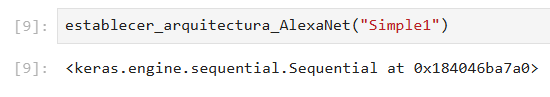
\includegraphics[width=0.99\textwidth]{img/ejemplo_simple1_estab_arq_propia.PNG}
    \caption{Ejecución función \textit{``establecer\_arquitectura\_AlexaNet''} para el modelo Simple1. Fuente propia.}
    \label{fig:ejemplo_simple1_estab_arq_propia}
\end{figure}
\FloatBarrier

En las funciones ``\textit{arq\_batch\_propia}'' y ``\textit{arq\_batch\_AlexNet}'', se comparan los distintos modelos mencionados previamente y distintos valores de \textit{batch size}. Para poder ser comparados los distintos valores de \textit{batch size}, se crea una lista con los valores y se añade como parámetro de entrada de las funciones. En este caso, tal y como se ha podido apreciar en el apartado de ``\textit{Resultados}'' de la memoria, se ha probado una lista de valores de [8, 16, 20, 32, 64]. Para cada modelo y valor de batch size, se obtienen unas métricas de entrenamiento concretas, las cuales se guardan en distintos archivos csv dentro de la carpeta ``Historicos''.

Por último, en la función ``\textit{neuronas}'', se realiza una comparación entre diferentes valores de neuronas para la capa oculta. Al igual que ocurría con el \textit{batch size}, se crea una lista con los distintos valores de neuronas y se añade como parámetro de entrada de la función. Los valores de neuronas a probar en este caso, han sido [512, 1024, 2048] y los resultados obtenidos se pueden ver en el apartado de ``\textit{Resultados}'' de la memoria. Para cada valor de neuronas, se obtienen unas métricas distintas que, también se guardan en la carpeta ``Historicos''.



\section{Instrucciones para la modificación o mejora del proyecto.}

Para que este trabajo pueda ser modificado en futuras ediciones, además de tener en cuenta la estructura del repositorio en GitHub mencionado previamente, se pueden considerar los siguientes puntos:

\begin{itemize}
    \item En este TFG, se han creado tres arquitecturas distintas (Simple1, Simple2 y Simple3) a partir de una CNN propia y de la CNN de AlexNet. En el caso de querer crear nuevas arquitecturas (para probar nuevas capas, nuevos parámetros, etc.), se puede tener en cuenta tanto la función ``\textit{establecer\_arquitectura\_propia}'' como ``\textit{establecer\_arquitectura\_AlexaNet}'' las cuales se encuentras perfectamente documentadas en los \textit{notebooks} de Python. 

    A la hora de modificar estas funciones, una recomendación podría ser mantener las CNN creadas y añadir nuevos modelos (``Simple4'', ``Simple5'', etc) con nuevas capas ocultas, o cambios en los parámetros. O, por el contrario, crear una nueva función con una nueva CNN y nuevos modelos basándose en las funciones ya creadas. 

    Sea como sea, hay que tener en cuenta que, en las siguientes funciones ``\textit{arq\_batch\_AlexNet}'', ``\textit{arq\_batch\_propia}'' y ``\textit{neuronas}'', donde se entrenan y evalúan los diferentes modelos, se emplean las funciones ``\textit{establecer\_arquitectura\_AlexaNet}'' y  ``\textit{establecer\_arquitectura\_propia}'' por lo que, deberán ser modificadas acorde a las nuevas arquitecturas creadas.

    \item Otra mejora, puede ser la implementación de transfer learning. El transfer learning o transferencia de aprendizaje, consiste en la reutilización de la información de un modelo ya pre-entrenado, para la realización de una tarea especifica. Es de gran utilidad en modelos donde no existe una gran cantidad de datos de entrenamiento \cite{diego23}. 

    Algunos modelos que se podrían probar disponibles en keras son: VGG (16, 19), MobileNet (v1, v2), DenseNet (121, 169, 201), entre otros \cite{diego23}. 

    A partir de estos nuevos modelos, se puede comprobar si la red neuronal realizada en este trabajo mejora o no.

    \item Estudiar más a fondo los diferentes parámetros de \textit{EarlyStopping} empleados durante el entrenamiento en las funciones ``\textit{arq\_batch\_AlexNet}'', ``\textit{arq\_batch\_propia}'' y ``\textit{neuronas}'' y probar parámetros nuevos. 

    \item Tal y como se ha comentado en el apartado de ``Líneas futuras'' de la memoria, otra mejora interesante para futuros desarrollos es el aumento de datos, es decir, incorporar nuevas imágenes en el desarrollo de esta red neuronal para mejorar el entrenamiento. 

    Las nuevas imágenes a introducir pueden ser, siguiendo la línea de este TFG, imágenes de CXT frontales de pacientes entre 1 y 5 años o, haciendo referencia a las ``lineas futuras'' y, para mejorar aún más el rendimiento del modelo, introducir imágenes de todos los rangos de edad y de otras vistas no frontales (como puede ser la oblicua, lateral, etc).
\end{itemize}


